\documentclass{article}

% Document Packages
\usepackage{hyperref}
\hypersetup{
    colorlinks=true,
    linkcolor=blue,
    filecolor=magenta,
    urlcolor=cyan,
}
\usepackage{geometry}
\geometry{
	a4paper,
	noheadfoot=true,
	left=1.0in,
	right=1.0in,
	top=1.0in,
	bottom=1.0in,
}

% Tikz and Figure Packages
\usepackage{caption}
\usepackage{amsmath} % aligned env
\usepackage{tikz}

\usetikzlibrary{decorations.pathreplacing}

%%%%%%%%%%%%%%%%%%%%%%%%%%%%%%%%%%%%%%%%%%%%%%%%%%%%%%%%%%%
%%% Titles
%%%%%%%%%%%%%%%%%%%%%%%%%%%%%%%%%%%%%%%%%%%%%%%%%%%%%%%%%%%

\title{Latex Tikz Examples, Model Timeline with Four Quadrants and Eight Panes}
\author{\href{https://fanwangecon.github.io/}{Fan Wang}\thanks{https://fanwangecon.github.io, repository: \href{https://fanwangecon.github.io/Tex4Econ/}{Tex4Econ}}}
\date{\today}

%%%%%%%%%%%%%%%%%%%%%%%%%%%%%%%%%%%%%%%%%%%%%%%%%%%%%%%%%%%
%%% Define Core Frame
%%%%%%%%%%%%%%%%%%%%%%%%%%%%%%%%%%%%%%%%%%%%%%%%%%%%%%%%%%%

\newcommand{\tikzframeeight}[7]{

  %%% 1. Define Figure Width and Height as Ratio of Page Width and Height
  % param 7 rescales, set same as every node/.style={scale=#7}
  \def\fgiw{#1*\textwidth*#7}  
  \def\fgih{#2*\textheight*#7}

  %%% 2. Cut Figure into Four Quadrants
  % fgiwm: breaks the left and right quadrants
  % fgihm: breaks the top and bottom quadrants
  \def\fgiwm{#3*\fgiw}
  \def\fgihm{#4*\fgih}

  %%% 3. Divide each quadrant into two parts, 8 parts
  % each quadrant now has small left edge or small right edge
  % fgile: break a small piece off left quadrant
  % fgire: break a small piece off left quadrant
  \def\fgile{#5*\fgiw}
  \def\fgire{#6*\fgiw}

  % left pane middle point, align horizontally middle pane
  \def\fgiwlm{\fgile*0.5 + \fgiwm*0.5}
  % right pane middle point, align horizontally middle in pane
  \def\fgiwrm{\fgiwm*0.5 + \fgire*0.5}

  % fgihtb: figure internal height top pane bottom
  % bottom 10 percent space of top pane space
  \def\fgihtb{\fgihm + \fgih*0.085 - \fgihm*0.085}

  % There is a flow line on top, limited text
  % three parts, left prior, right after, middle current.
  % current in two parts, shock realization and choices.
  % In top part, span charts, simple text
  % in bottom part, sufficient height to allow for detailed text
  % descriptions.

  % Bottom and top lines
  \draw [solid] (0, \fgih) -- (\fgiw, \fgih);
  \draw [solid] (0, 0    ) -- (\fgiw, 0    );

  % Left and right lines
  \draw [solid] (0,     0) -- (0,     \fgih);
  \draw [solid] (\fgiw, 0) -- (\fgiw, \fgih);

  % verticle middle line
  \draw [solid] (\fgiwm, 0) -- (\fgiwm,   \fgih);
  % horizontal middle line (divide text and flow)
  \draw [solid] (0, \fgihm) -- (\fgiw,   \fgihm);

  % left border last period
  \draw[dashed] (\fgile, 0  ) -- (\fgile,   \fgih);
  % right border next period
  \draw[dashed] (\fgire, 0  ) -- (\fgire,   \fgih);

  % %
  % \draw[loosely dotted] (0, 0.575*\fgih) -- (\fgiw, 0.575*\fgih);
  % \draw[loosely dotted] (0, 0.350*\fgih) -- (\fgiw, 0.350*\fgih);
  \node[align=center] at (0.5*\fgile,             0.900*\fgih) {last\\period};
  \node[align=center] at (0.5*\fgiw,              0.900*\fgih) {current period};
  \node[align=center] at (0.5*\fgire + 0.5*\fgiw, 0.900*\fgih) {next\\period};

  \node[align=center] at (\fgiwlm, \fgihtb) {shocks};
  \node[align=center] at (\fgiwrm, \fgihtb) {asset choices};
}

\begin{document}

\maketitle

Generate a eight pane model timeline tikz structure. The proportional sizes of each pane is determined by parameters, and are porportional to pages. The timeline structure is meant to be used for dynamic models with previous, current and next period. Shocks arise and decisions are made in the current period. 


\section{Empty Frames with Eight Panes}

The idea is that the top panes would show overall model timeline. The bottomw below horizontal line spaces could have equations that provide more information sufficiently about what is happening in timeline above. 


\begin{center}
  \begin{tikzpicture}[scale=1.0, every node/.style={scale=1.0}]
    \tikzframeeight{1}{0.25}{0.5}{0.35}{0.125}{0.875}{1.0}
  \end{tikzpicture}
\end{center}

\begin{center}
  \begin{tikzpicture}[scale=1.0, every node/.style={scale=0.5}]
    \tikzframeeight{1}{0.25}{0.5}{0.35}{0.125}{0.875}{0.5}
  \end{tikzpicture}
\end{center}

\begin{center}
  \begin{tikzpicture}[scale=1.0, every node/.style={scale=0.5}]
    \tikzframeeight{1}{0.25}{0.5}{0.35}{0.125}{0.875}{0.30}
  \end{tikzpicture}
\end{center}

% \begin{center}
%   \begin{tikzpicture}[scale=1.0, every node/.style={scale=0.5}]
%     \tikzframeeight{0.5}{0.125}{0.4}{0.35}
%   \end{tikzpicture}
% \end{center}
  
% \begin{center}
%   \begin{tikzpicture}[scale=1.0, every node/.style={scale=1.0}]
%     \tikzframeeight{0.6}{0.20}{0.4}{0.35}
%   \end{tikzpicture}
% \end{center}

% \begin{center}
%   \begin{tikzpicture}[scale=1.0, every node/.style={scale=1.0}]
%     \tikzframeeight{0.3}{0.10}{0.4}{0.35}
%   \end{tikzpicture}
% \end{center}

% \begin{center}
%   \begin{tikzpicture}[scale=1.0, every node/.style={scale=1.0}]
%     \tikzframeeight{1}{0.15}{0.5}{0.5}
%   \end{tikzpicture}
% \end{center}

\end{document}
